\ifdefined\THESIS
    \chapter{\uppercase{Evaluation}}
    \label{chap:eval}
\else
    \section{Evaluation}
\fi

We evaluate the system against several baseline implementations, and evaluate
how the performance of the system varies with the number of contacts a user has
and how many FriendlyLocation chooses to use.
We used five-fold cross validation on the target users to evaluate the system.
We evaluated the FriendlyLocation system against the 249,584 target users.

\emph{define aed and acc}

\begin{figure}[tb]
\centering
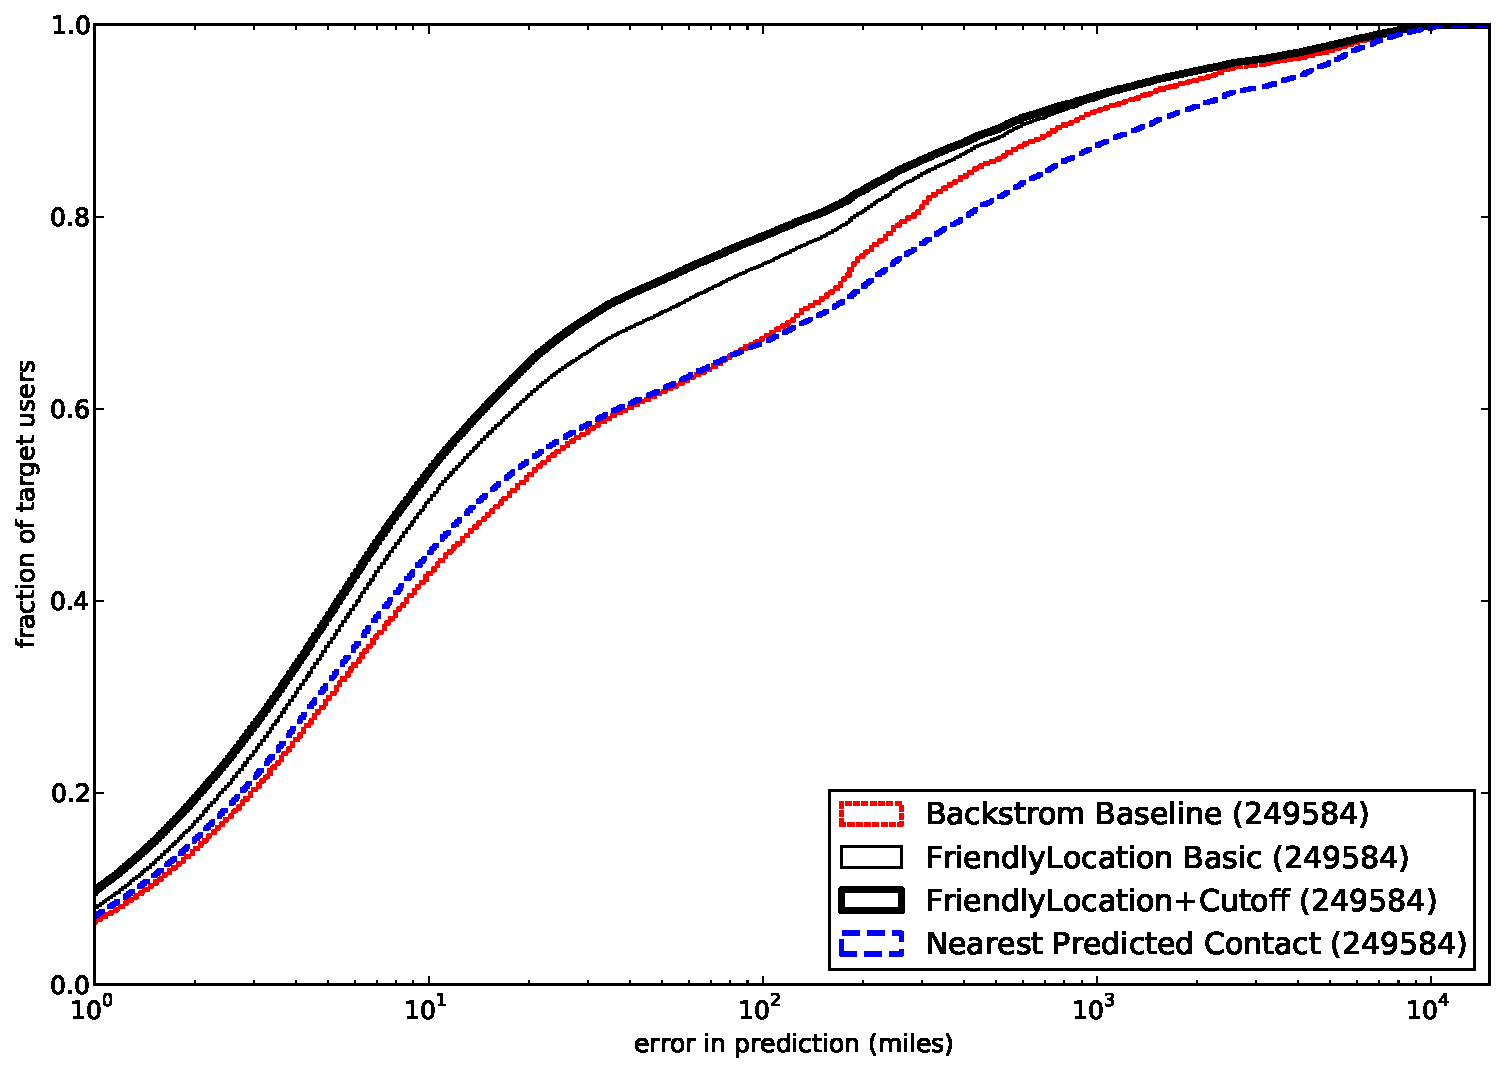
\includegraphics[width=\linewidth]{figures/fl_basic.pdf}
\caption{
    FriendlyLocation against several baseline systems.
}
\label{fig:baseline}
\end{figure}

\begin{table}[tb]
\centering
\begin{tabular}{l  r r r r}
    Model & aed@60 & aed@80 & aed@100 & acc@25 \\
    \hline
    Baseline & 8.41$\pm$.039 & 40.8$\pm$.20 & 426$\pm$3.8 & 55.7\%$\pm$.09\% \\
    Nearest & 7.50$\pm$.072 & 47.8$\pm$.52 & 573$\pm$4.5 & 56.9\%$\pm$.17\% \\
    FriendLoc Basic & 5.43$\pm$.030 & 21.4$\pm$.15 & 359$\pm$3.8 & 63.9\%$\pm$.11\% \\
    FriendLoc+Time Zone & 5.46$\pm$.025 & 21.4$\pm$.11 & 354$\pm$4.8 & 63.9\%$\pm$.06\% \\
    FriendLoc+Location & 4.78$\pm$.025 & 16.6$\pm$.22 & 331$\pm$3.1 & 66.5\%$\pm$.08\% \\
\end{tabular}
\caption{
    Results of our location prediction system when compared to a baseline.
    The value after the $\pm$ is the standard deviation from the five-fold
    cross-validation.
    Including the target user's time zone information does not improve the
    results, but using the target user's reported location, if they gave one,
    makes for significantly better results.
}
\label{tab:results}
\end{table}

\section{Prediction}
We investigate several implementations of the FriendlyLocation system:
\begin{description}
\item[Baseline] This is based on the MLE estimator presented in
    \cite{backstrom2010find}. Some changes to the system had to be made to make it
    work on Twitter's directed graph. (Facebook friendships are always
    reciprocal.)
\item[Nearest Contact] This predictor chooses the location of the contact that
    the tree regressor picks as the closest contact.
\item[FriendlyLocation Basic] This is the system described in the previous
    section with only information from the locations of contacts.
\item[FriendlyLocation + Time Zone] This is the system described in the previous
    section plus the target user's time zone information.
\item[FriendlyLocation + Location] This is the system described in the previous
    section plus the target user's reported location is included in the
    estimation.
\end{description}

Our basic FriendlyLocation system predicts the location within 25 miles 63.9\% of
the time.
%
Our basic system preforms significantly better than the baseline implementations.
%
Unfortunately, when the predictor is wrong, it can be very wrong. \emph{More here.}
%
%The comparison to the omniscient predictor shows that there is room for improvement.
%
%Many users who have an incorrectly predicted location have at least one contact
%that is closer than the incorrectly predicted location.


\section{Additional Information}
Many Twitter users fill out the text-based location field.
%
If this user-reported data is good, there is no reason to spend time
crawling their contacts.
%
It would be nice to use this information when predicting location, but
the target users we used to do the evaluation are less concerned about
the privacy of their location information than the average Twitter user.
%
As a result, they tended to give more precise information in the location
field of their user profile than other users.
%
We assume that the locations supplied by the contacts are more
representative of normal Twitter users so we added noise to the locations
of the target users to make the distribution of the quality of their
locations would match the quality of the contacts.
%
First, we sorted all the target users and all the contacts by their
PLE(predicted location error).
%
Next, we looked at each percentile of the target users and compared
their PLE to the PLE for that percentile in the contacts.
%
For each of the target users, we moved the user's location based on
reverse geocoding away from the user's actual median location based on the
difference between the PLEs.
%
For example, the median PLE for a target user was 5.9 miles, and the median
PLE for a contact was 6.7 miles.
%
This means that we need to add .8 miles of noise to a target user
with a PLE of 5.9 so that the quality of the geo-located target user's location
would match the quality of normal Twitter users.
%
We also removed the location field from 17\% of the target users to
make the proportion of target users with a location match the general
Twitter population.

\emph{discuss adding other factors}
\emph{do we want to do us-only evaluation?}

The final step of the evaluation is to investigate if FriendlyLocation would
work with a smaller number of profiles than 25.
%
\emph{eval for small number of hand-picked and random contacts}
%
In general, using more contacts ought to produce better results.
%
Although we limited the crawler to 25 randomly-picked contacts per target
user, if FriendlyLocation is going to be used as part of a larger system, the
crawler should pick users based on relationship type before crawling.

%Before removing contacts without location information, we sorted the users into
%groups based on the number of contacts the had.
%Next, we ran the FriendlyLocation predictor against each of them.
%Figure~\ref{fig:LulResults} shows the results of prediction.
%The quality of the results from the predictor was lower for users with fewer
%than 50 contacts; however, as contacts increased beyond that, it had no
%significant effect on the results.


